\chapter{Background} % Main chapter title

\label{Chapter2} % Change X to a consecutive number; for referencing this chapter elsewhere, use \ref{ChapterX}

Computers have a long history of being built to serve a particular purpose, often compromising some aspects of the system to bolster others.
Chapter \ref{sec:SpecializationOfComputers} discusses the history of how computers were built for a particular function, and how the advancement of technology has brought the \enquote{Personal Computer} seen know today.
Chapter \ref{subsec:PowerOfTheDesktop} discusses the benefits of a desktop computer, Chapter \ref{subsec:ConvenienceOfTheLaptop} discusses the benefits and drawbacks of a laptop computer, and Chapter \ref{subsec:RiseOfTheGamingLaptop} discusses the rise of the gaming laptop and the closing gap between power and portability at the cost of increased price.
Chapter \ref{sec:ThinClients} briefly discusses thin clients, a corporate solution for remote access to a computer.
Chapter \ref{sec:ApplicationToModernDay} introduces current world wide context that has an impact on the computing world and the need for power and portability.

\section{Specialization of Computers}\label{sec:SpecializationOfComputers}

In the age of punch cards and monolithic computers the size of entire rooms, it was expected of a computer to only be capable of serving a single function.
Before the technology could be miniaturized, every single computer had to be specialized for the job at hand.
As time passed and technology progressed, a single computer could be produced that served multiple functions as well as be adaptable programmable to handle new tasks that were not considered when the machine was originally built.
This gave rise to what was known as \enquote{Autonomic Computing}, a system of characteristics that are built into a computer to help it self-manage it's resources and adapt to it's administrator's requirements without the need to be redesigned for it's new purpose \citep{AutonomicComputing}.
Autonomic Computing was designed to combat the exponential complexity crisis that came from the widespread availability of computers in different disciplines, since now anyone who could afford a computer could program it for any purpose.
As new use cases were found for computers in day-to-day life and new technologies were being developed to interface with the world around us, the need for componentization became ever more apparent.
Researchers at IBM knew that the best way to address the looming problem of runaway complexity in computers was to develop a way for the computers to automatically interface with any new components that are installed, and to configure itself to only use what is necessary for the job at hand \citep[p.~43]{AutonomicComputing}.
This allowed hardware and software developers to focus on building their products to work with a common standard rather than having to manually integrate their products with every computer.

Once the idea of modularity began to take hold in the computer industry, attention was turned once again towards specializing individual computers.
Now that a computer's physical footprint can be minified, and peripheral components can be added and removed without a complete reengineering of the device, a single computer can be optimized to handle a single task without the overhead cost of building a monolithic computer \citep{Burbeck2007ComplexityAT}.
Now a computer can be specialized to serve a particular purpose or set of purposes while keeping development time comparatively short.
The world has seen this realized through numerous applications such as cell phones, designed to be user-friendly portable devices, computing clusters, built for high-performance computing, or even internet routers, which are built to be a plug-and-play solution for a problem posed to users of all levels of familiarity with computers.
Without this idea of Autonomic Computing, each of these devices would have to be reengineered from the ground up every time a new use case was developed.

This leads into the specialization of home computers in from the perspective of a consumer.
It used to be that a \enquote{home computer} was a device that was bought off the shelf as-is and served it's purpose.
Now a home computer can be a desktop PC that can be upgraded with time and seldom moves from it's place, or it could be a laptop that is portable and easy to cary around.
These specializations bring more choices for the consumer to pick a computer that best suits their needs, but they often come with compromises.

\subsection{Power of the Desktop}\label{subsec:PowerOfTheDesktop}

The classical manifestation of a personal computer is the desktop computer.
Known for it's componentization, user repairability, and direct connections to power and the network, desktop computers are the best option for a user looking for a workhorse system.
Pieces of the computer could be bought separately, and single parts could be upgraded or replaced by anyone will a little hardware knowledge.
Even though they aren't very portable, desktop computers allow consumers to access greater processor power for a lower cost compared to portable devices \citep{Meyer20145RS}.
Due to this, a desktop PC is often seen at one's home or place of work hardwired to the wall where it remains unmoving unless it needs upgrading, cleaning, or repairs.
Adding on the fact the desktop is modular, it can be easily customized to fit any user's needs, as well as enable particular parts to be replaced or upgraded without needing to rebuild the entire system.

While desktops were the staple of personal computers for decades, advancing technology and the rising need of portability and flexibility has led to the growth of laptops.


\subsection{Convenience of the Laptop}\label{subsec:ConvenienceOfTheLaptop}

As the world moved towards a more mobile lifestyle, the laptop shifted from being a luxury to being a necessity.
People began to need computing power on the go, whether it be for working remotely, attending classes and following along, or simply needing more power than their phone can offer.
Companies began to take note too and started building applications to work fully within a web browser, such as Google's implementation of Google Docs, allowing users to edit documents on the go without having to install software like Microsoft Word directly to their computers.
This shift towards mobility provided the general public the ability to be more flexible with how they used computers, no longer requiring them to dedicating a spot in their house to be taken up by a desktop computer.

Reducing the barrier to entry for computers, such as the knowledge to buy the computer the best fits their needs and the restrictions that come with setting up and keeping a desktop, led to the widespread adoption of laptops.
In fact, by 2021, laptops accounted for 80\% of total computer sales \cite{idc_2021}.
For most consumers, the laptop is all they need; it may not have the raw power of a desktop, but it handles everything they need it to do.
The biggest limiting factor then becomes technology, with manufacturers constantly trying to minimize existing desktop technology into the footprint of a laptop while keeping energy efficiency high enough to be feasible in a mobile device.


\subsection{Rise of the Gaming Laptop}\label{subsec:RiseOfTheGamingLaptop}

All computer products are a balance, it simply isn't possible to have the perfect combination of portable, powerful, serviceable, and cheap.
While desktops focus on power and serviceability, laptops often focus portability at the expense of other traits\todo{Theres a word at the tip of my tounge thats a lot better here dangit}.
As mobility becomes ever more important, gaming laptops have become more popular to bring power to the portable form factor.
This understandably comes with a cost, with the literal cost of a gaming laptop being the most obvious compromise.
The componentization of such a laptop also often takes a hit with parts being directly soldered to the motherboard, reducing a user's options for repairs or upgrades.
It is more expensive, and often less user-serviceable, to buy a gaming laptop that has the same performance of a desktop computer -- but given that it is an all-in-one device, it's portability gives it a niche that a desktop cannot hope to rival.
The compromise presented by a gaming laptop helps close the gap between power and portability, but it still falls short of being an all around good solution.


\section{Thin Clients}\label{sec:ThinClients}

\begin{wrapfigure}{r}{0.375\textwidth}
  \centering
  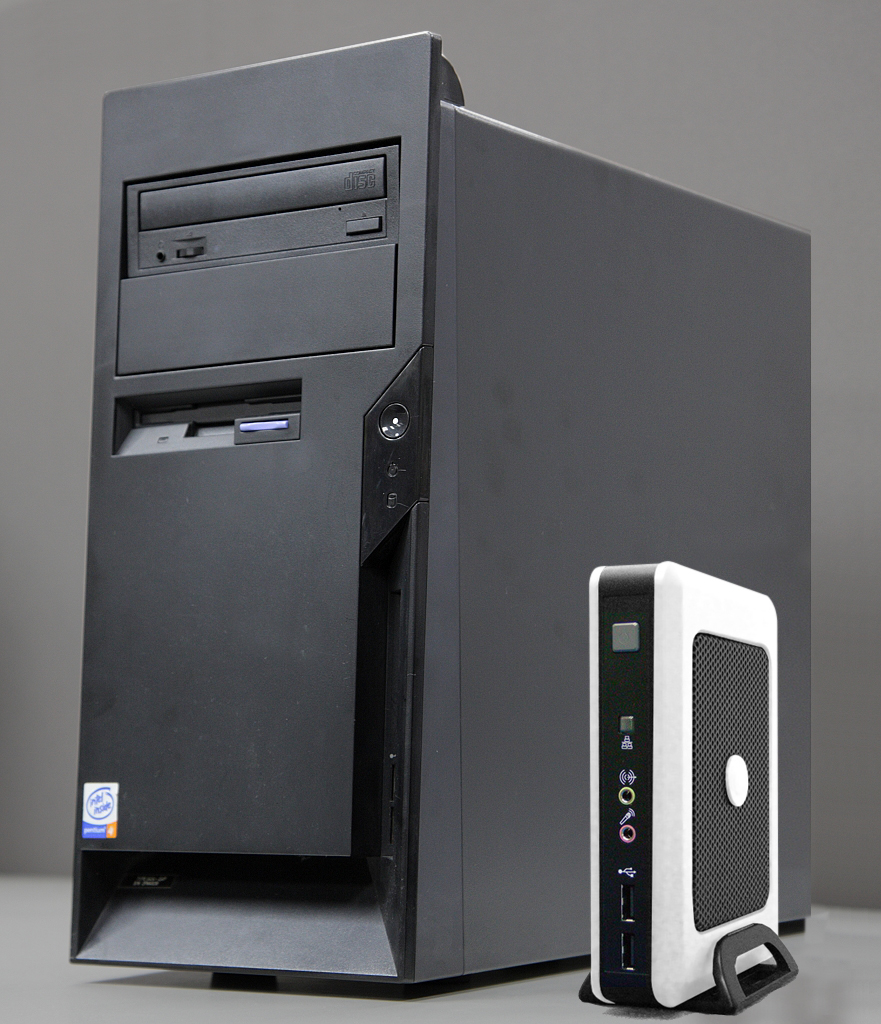
\includegraphics[width=0.3\textwidth]{Figures/ClientronU700}
  \caption[Thin Client]{A thin client next to a traditional desktop computer \cite{ImageThinClient}.}
  \label{fig:ThinClient}
\end{wrapfigure}

On the corporate side of computing, the solution for portability has been the thin client.
Rather than integrating the power of a desktop to a portable machine, a thin client will connect to a powerful server and provide a thin interface to the user.
This allows the user to utilize the power of the host machine from a cheap computer that usually doesn't have enough power to be used as a standalone computer.
Because of it's low power, the thin client cannot be used as a standalone computer, but it's low cost and portability make it a great solution for a corporate user.
While these clients work well for simple interfacing tasks such as data entry or system management, they are not designed to be used for complex tasks that require quick response times or graphical fidelity.


\section{Application to Modern Day}\label{sec:ApplicationToModernDay}

In 2022, the world is currently going through some chaotic times that demand flexibility and adaptability like it hasn't faced before.
From the COVID-19 pandemic to massive chip shortages and supply line disruptions, people are now more than ever looking for a way to be flexible in their work and personal lives now and in the future.
The COVID-19 pandemic has forced people to be able to operate remotely, whether that be for work, school, or communicating with friends and family \cite{levanon_2020}.
Many office workers used to working on a desktop computer onsite are now needed to work from home, or classes usually taught in person are now held remotely \cite{ASU_covid_19}.
This shift to remote operation has fueled the need for mobile computers, many of which need to be powerful enough to handle the workload of a desktop computer from anywhere in the world.
The global chip shortage is also causing issues for the purchase of new devices \cite{chipshortage_jpmorgan}.
Parts which are usually readily available for purchase are out of stock with months of delay on back order.
Resellers are taking advantage of the situation by hiking prices to two or three times the original listing price, and it's become harder than ever to build a new PC \cite{tamarov_2021}.
All of these factors combined lead to a very difficult situation for anyone looking to purchase a new computer or parts for their existing computer.

It doesn't make sense to build or purchase a powerful PC for use at home and another power laptop to handle working on the go, especially with rising prices, so many people are moving to exclusively powerful laptops or looking for other solutions.
